\documentclass[10pt]{article}
\usepackage[margin=1in]{geometry}
\usepackage{titlesec}
\usepackage{graphicx}
\pagenumbering{gobble}

% Title formatting
\titleformat{\section}{\large\bfseries}{\thesection}{1em}{}
\titleformat{\subsection}{\normalsize\bfseries}{\thesubsection}{1em}{}

\begin{document}

\begin{center}
    {\LARGE \textbf{Accelerating BFS algorithms on FPGA}} \\[10pt]
    \textbf{Ethan Gabizon (ehg54), Tomas Choi (tic3), Dylan Lee (dl634)}
\end{center}

\section{Introduction}
\noindent We implement an optimized breadth first search algorithm on FPGA. Traditional graph algorithms 
are difficult to implement efficiently on a general-purpose CPU because of their irregular memory 
access patterns. They also tend to be memory-intensive rather than compute-intensive because they 
involve traversals, in which values get read and then almost immediately written back to memory with 
very little compute in between. We use the Alveo U280 card and leverage its high-bandwidth memory to 
accelerate BFS. First, we modify the representation of the BFS problem by using the coordinate format.
Then, we implement a BFS traversal over a graph as a series of sparse-matrix-dense-vector multiplies; this 
approach of implementing graph algorithms with linear algebra is known as GraphBLAS. We optimize this BFS 
by instantiating multiple processing elements that can concurrently perform SPMV on different rows. To 
benchmark our designs, we use graphs from the SuiteSparse Matrix Collection. We compare our optimized designs
against the unoptimized FPGA design.

\section{Background}
\subsection{Alveo U280 FPGA Platform}
\noindent For the labs, we use the Zedboard, but for this final project we use the Alveo U280 card. The Alveo U280 
card is a data center accelerator card containing a more powerful FPGA due to its capacity, bandwidth, and 
power efficiency. Figure~\ref{fig:u250} shows the Alveo block diagram for the U250 card (it is still relevant for 
the description of the U280 card). The FPGA is divided into two partitions, shell and user. The shell partition 
is a static region that provides the basic control and communication for things like PCIe connectivity, board 
management, clocking, and reset. The user partition is a dynamic region that contains the user compiled binary,
so the hardware that we synthesize. There is a PCIe interface for the host and FPGA to communicate with each
other. The PCIe interface will allow the transfer of data between the host and the device memory, where the device 
memory could be PLRAM, HBM, or DDR. \newline

\begin{figure}[h!]
  \centering
  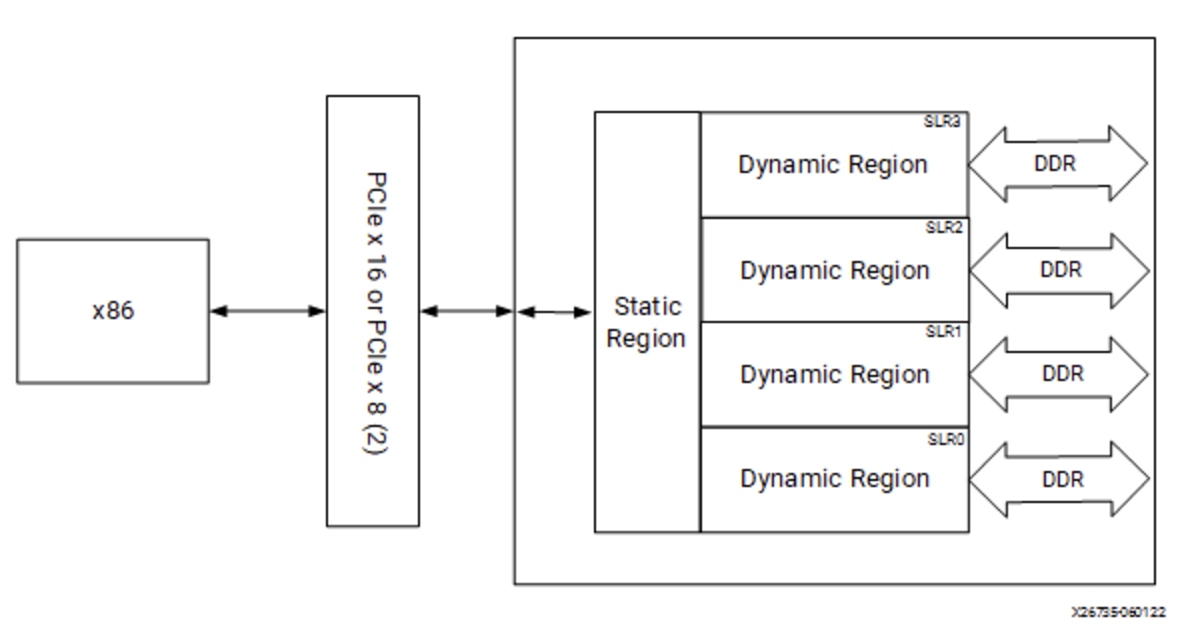
\includegraphics[width=0.5\textwidth]{u250.png}
  \caption{U250 Block Diagram}
  \label{fig:u250}
\end{figure}

\noindent For our project, we only used HBM. High bandwidth memory is a high performance memory technology that 
allows for massive memory bandwidth by exposing multiple memory channels to the processing units. Figure~\ref{fig:hbm} 
shows the HBM subsystem in the U280 card. It contains two HBM stacks, and each has 16 pseudo channels. Above the pseudo 
channels, there are 16 memory channels that each control two pseudo channels. Then, there is a switch network for 
every two memory channels that exposes 4 AXI interfaces, so in total there are 32 AXI ports. For our project, we 
use a maximum of 18 of these because our designs range from using one HBM channel to 16 just for coordinate data. 
It is important to emphasize that HBM allows our memory bound workload of BFS to be pushed computationally. 

\begin{figure}[h!]
  \centering
  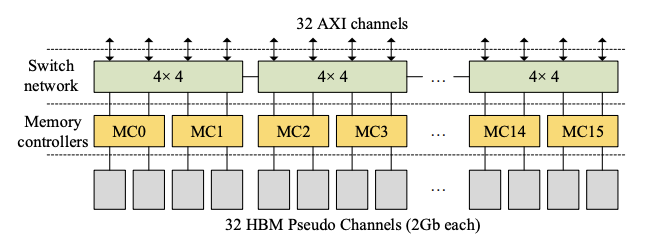
\includegraphics[width=0.5\textwidth]{hbm.png}
  \caption{HBM Subsystem in U280 Card}
  \label{fig:hbm}
\end{figure}

\subsection{Vitis Software}


\subsection{HLS Directives}
To optimize our design, we use multiple HLS directives: dataflow, interface, loop tripcount,
array partition, pipeline, and unroll. For this report, we focus on the ones that most students 
in ECE6775 are not familiar with. First, the \textbf{dataflow} pragma enables task-level parallelism. 
This allows functions and loops to overlap in their operation. If there are any consumer and producer 
relationships in the dataflow region, then their respective functions will need to wait for each 
other. If there are none, then all of the functions could run concurrently. The Vitis HLS tool 
will try to minimize the overall latency and improve concurrency by starting operations as soon 
as data is available. Second, the \textbf{interface} pragma specifies how RTL ports are created from 
the function definition during interface synthesis. This pragma defines how data is passed between 
the design and the external world. It determines the communication protocol, data handling, and 
optimization of memory access for ports, arrays, and variables in the design. Lastly, the 
\textbf{loop tripcount} directive is used to specify the minimum, maximum, and average trips that a 
loop might take. This directive is only used for analysis and it does not actually affect the synthesis 
results. We used it to specify the trip count of our variable bound loops to have better estimates of 
latency while optimizing our design. \newline

\section{Problem Description}

\subsection{BFS}
We begin by giving a high level overview of BFS. Breadth First Search is a graph traversal algorithm
in which you start at a node and traverse all of its adjacent nodes. Once all the adjacent nodes are visited,
then those nodes' adjacent nodes are visited. Figure~\ref{fig:bfs_graph} shows an example traversal order. 
The common opposite to Breadth First Search is Depth First Search where you start at a node, traverse to an 
adjacent node, and traverse all nodes reachable through that adjacent node before moving on to the next adjacent
node. \newline

\begin{figure}[h!]
  \centering
  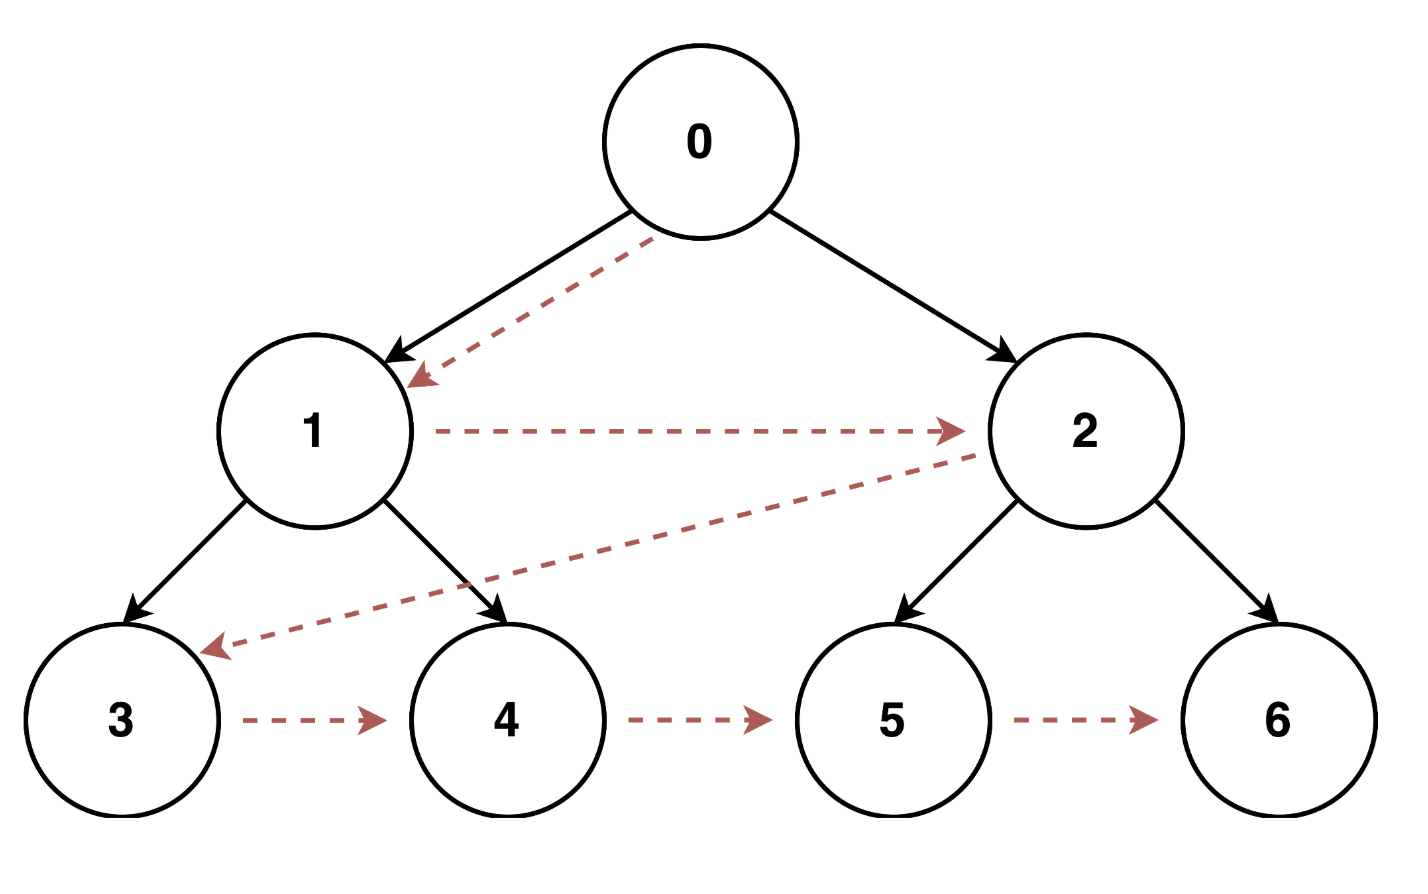
\includegraphics[width=0.5\textwidth]{bfs_graph.png}
  \caption{BFS Example Traversal Order}
  \label{fig:bfs_graph}
\end{figure}

\subsection{BFS with Linear Algebra}
Instead of the traditional way to implement graph algorithms, we take advantage of the fact that a graph can 
be represented as a matrix to which linear transformations can be applied to perform these graph operations.
We use sparse matrix multiplication to perform our BFS algorithm. This is a common way to perform BFS as documented
in the GraphBLAS specification. We can represent graphs using adjacency matrices in which the value at (i, j) in the 
matrix represents the presence of an edge and possibly a weight between nodes i and j. In our case, these weights will
be 0 or 1 to simply represent the presence of an edge. Using these matrices, we can perform BFS by iteratively conducting 
matrix vector multiplication with the adjacency matrix and a vector that represents the frontier, where a 1 in the ith 
in the frontier means that node i will be explored. Figure~\ref{fig:adj_matrix} shows the way in which the example in 
Figure~\ref{fig:bfs_graph} is mapped to an adjacency matrix that facilitates matrix vector operations. \newline

\textit{TODO: Should we add an example on how the iterations work? Like perform an spmv and see that it looks at all the 
nodes in that breadth?}

\begin{figure}[h!]
  \centering
  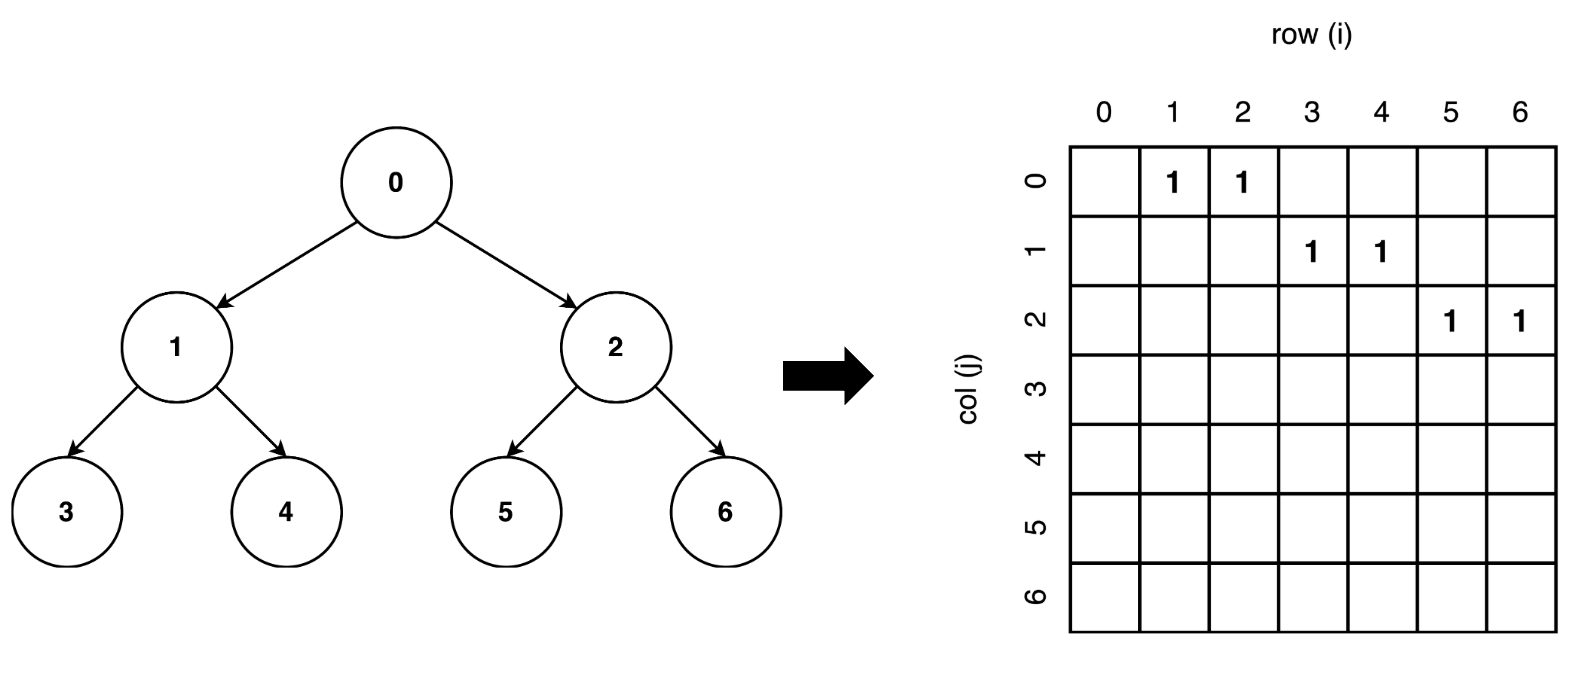
\includegraphics[width=0.5\textwidth]{adj_matrix.png}
  \caption{Adjacency Matrix Representation of Graph}
  \label{fig:adj_matrix}
\end{figure}

\subsection{Architecture}

\textit{This section should provide a detailed description of the applications or
automation algorithms/tools realized in this project. Think critically about the important items to
mention in order for the reader to understand how your design works without having to look into any
code. For example, what are the inputs and outputs of the application (or architecture), what are the
major steps (or modules), and what are the key characteristics (e.g., sources of parallelism and operational intensity) of these steps? It would be useful to include small examples, block diagrams, formulas,
or other visualizations to help explain your techniques. Please do not include detailed information
about your source code as your report should be at a high level.}


\section{Implementation}
\textit{This section should describe how you implemented and optimized your designs. For
example, did you take advantage of any third-party libraries? Which software and/or hardware blocks
are included in your design, and what hardware device (if any) did you target? Please also describe
how you optimize the design. If you use more than one optimization methods, please summarize them
in this section and later compare their impacts in the evaluation section regarding different aspect (e.g.,
performance, resource usage, accuracy). In most cases, it would be helpful to include block diagrams
of your implementation illustrating the flow of data through your design, the interconnection between
different hardware blocks, and whether certain blocks are pipelined or parallelized. As in the previous
section, providing meaningful visualizations would help the reader better appreciate your work.}

\subsection{Base Design}


\subsection{8 PE Design}


\subsection{16 PE Design}


\section{Testing}


\section{Evaluation}
\textit{Students should describe the experimental setup used to evaluate their design. Students
should describe the data inputs used to evaluate their design and provide an analysis of the achieved
results. The results should be clearly summarized in terms of tables, text, and/or plots. Please provide
qualitative and quantitative analysis of the results and discuss insights from these results. Results may
include (but are not limited to) the execution time of an algorithm, hardware resource usage, achievable
throughput, and error rate. It would be interesting, for example, to discuss why one design is better
than another, why one design achieves a higher metric than another, or how you trade-off one metric
for another. Consider going into detail for one particular instance of your experiment and analyze how
it achieves the given results}


\section{Project Management}
\textit{This section should clearly identify the work division among the students in
the group using a project timeline that lists the tasks and milestones of the project, the member(s) of
the group responsible for each task, and the actual completion date of each task. This section should
contain a description of how the overall project progressed and any successes and/or challenges during
the course of the project.}

\section{Conclusion}

\textit{This section should provide a concise summary of the algorithms, implementation, and results. Please also summarize the lessons you learned in the course of
the project and acknowledge the additional help you received from the course staff or other students}


\end{document}